\documentclass[11pt, oneside]{article} 
\usepackage{geometry}
\geometry{letterpaper} 
\usepackage{graphicx}
	
\usepackage{amssymb}
\usepackage{amsmath}
\usepackage{parskip}
\usepackage{color}
\usepackage{hyperref}

\graphicspath{{/Users/telliott_admin/Tex/png/}}
% \begin{center} 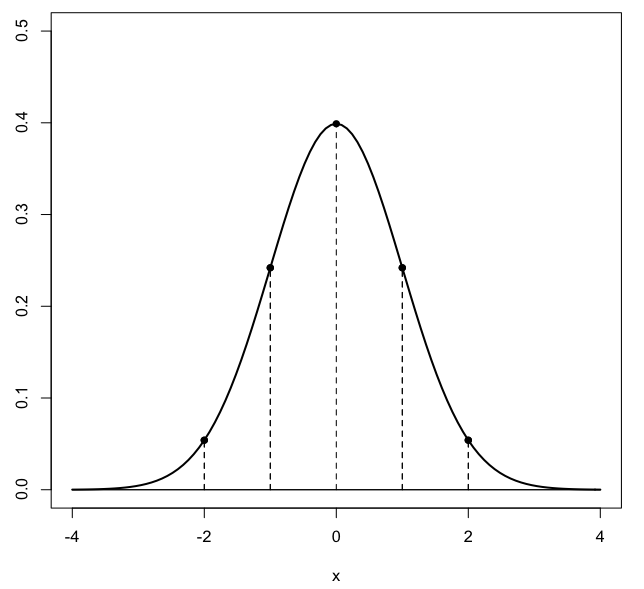
\includegraphics [scale=0.4] {gauss3.png} \end{center}

\title{Stokes Theorem}
\date{}

\begin{document}
\maketitle
\Large

\[ \oint_C \mathbf{F} \cdot d \mathbf{r} = \iint_S ( \nabla \times \mathbf{F}) \cdot \hat{\mathbf{n}} \ dS \]
Stokes' theorem applies to a curve in space (it does not have to lie in a plane).  The theorem says that the work going around a closed curve is equal to the integral over \emph{any surface} with that curve as its boundary, of the component of the curl of $\mathbf{F}$ normal to the surface. 

An alternative form (using the fact that $\mathbf{dr} = \langle dx,dy,dz \rangle$, and computing the curl $\nabla \times \mathbf{F}$) is

\[ \int_C M \ dx + N \ dy + P \ dz = \iint_R   \ \ \langle P_y-N_z,M_z-P_x,N_x-M_y \rangle \  \  \cdot  \hat{\mathbf{n}} \ dS \]

When Stokes' theorem is applied to a region in the $xy$-plane, $\hat{\mathbf{n}} = \hat{\mathbf{k}}$, so only the third term of the curl is non-zero, and $dS = dA$.  On the left-hand side $dz=0$, so this just reduces to

\[  \int_C M \ dx + N \ dy  = \iint_R \ (N_x-M_y) \ dA \]

which is Green's theorem for work.

\subsection*{example}

State the theorem:
\[ \oint_C \mathbf{F} \cdot \mathbf{r} = \iint_R (\nabla \times \mathbf{F}) \cdot \hat{\mathbf{n}} \ dS \]
By the usual reasoning, since $d\mathbf{r} = \ <dx,dy,dz>$, the left-hand side is
\[ P \ dx + Q \ dy + R \ dz \]
Now, suppose we have 
\[ \mathbf{F} = \ <z,x,y> \]
and $C$ is the unit circle in the $xy$-plane,
then 
\[ P \ dx + Q \ dy + R \ dz = \oint_C  z \ dx + x \ dy + y \ dz =   \oint_C x \ dy \]
Parameterize
\[ C =
\left\{
	\begin{array}{l}
		x  = \cos t  \\
		y  = \sin t
	\end{array}
\right.
\]
we have
\[ \oint_C x \ dy = \int_0^{2\pi} \ \cos t \ \cos t \ dt \]
\[ = \frac{1}{2}(t + \frac{1}{2} \sin t) \ \bigg |_0^{2\pi} = \pi \]
For the surface, we can use anything that passes through $C$, let's use the paraboloid for fun.
\[ z = 1 - x^2 - y^2 \]
We need the curl of $\mathbf{F} = \ <z,x,y> $
\[ \nabla \times \mathbf{F} = \ < 1,1,1> \]
We need
\[ \hat{\mathbf{n}} \ dS = \ <-f_x,-f_y,1> \ dx \ dy =  \ <2x,2y,1> \ dx \ dy \]
so
\[ \iint_R (\nabla \times \mathbf{F}) \cdot \hat{\mathbf{n}} \ dS =  \iint_R \ 2x + 2y + 1 \ dx \ dy \]
Again, $C$ is the unit circle in the $xy$-plane.  To save effort, we can notice that 
\[ \int x \ dx = \overline{x} \]
What is the \emph{average} value of $x$ over the unit circle?  It is just equal to $0$.  The same thing is true for the second integrand (reverse the order of integration).  So we have just
\[ \iint_R \  1 \ dx \ dy = \pi \]
which matches what we had above.

Suppose we hadn't seen this.  We could just do
\[ \int_{x=-1}^{1} \int_{y=-\sqrt{1-x^2}}^{\sqrt{1-x^2}} \ x \ dy \ dx \]
\[ = \int_{x=-1}^{1} 2 \sqrt{1-x^2} \ x \ dy \ dx \]
\[ = - \frac{2}{3} \ (1-x^2)^{3/2} \ \bigg |_{-1}^1 \]
At both bounds, $1-x^2 = 0$, so the whole thing is $0$.

Stokes Theorem is:
\[ \oint_C \mathbf{F} \cdot \mathbf{r} = \iint_R (\nabla \times \mathbf{F}) \cdot \hat{\mathbf{n}} \ dS \]

\subsection*{Problem 1}

Given 
\[ \mathbf{F} = \langle yz,xz,xy \rangle \]
Show that the integral
\[ \oint_C yz \ dx + xz \ dy + xy \ dz = 0 \]
over \emph{any} closed curve $C$.

One way to do this is to guess the potential function for which $\mathbf{F} = \nabla f$.
\[ f(x,y,z) = xyz \]
fulfills this criterion.  Since this is true, the curl of $\mathbf{F}$ must be zero.  By Stokes theorem, the integral is zero for any closed curve $C$.

A second approach is to actually calculate the curl
\[ \nabla \times \mathbf{F} = \langle R_y - Q_z, P_z - R_x, Q_x - P_y \rangle \]
\[ = \langle x - x, y - y, z - z \rangle = \langle 0, 0, 0 \rangle \]
and the dot product with \emph{any} $\hat{\mathbf{n}}$ is zero.

\subsection*{Problem 2}
Evaluate
\[ \oint_C (y + 2z)dx + (x + 2z)dy + (x + 2y)dz \]
where $C$ is the intersection of the unit sphere $x^2 + y^2 + z^2 = 1$ with the plane $x + 2y + 2z = 0$.  This looks fairly hard at first.  How to parameterize this curve?  But we start by calculating
\[ \nabla \times \mathbf{F} = \langle 2 - 2, 2 - 1, 1 - 1 \rangle = \langle 0, 1, 0 \rangle  \]
What is $\hat{\mathbf{n}} \ dS$?  Our surface is a part of the plane.  Notice that $(0,0,0)$ is a solution of the equation for the plane, so it goes through the origin.  Therefore, the intersection is a circle of radius $1$.  The plane has normal vector $\mathbf{n} = \langle 1,2,2 \rangle$ and \emph{unit normal} $\hat{\mathbf{n}} = 1/3 \ \mathbf{n}$ so
\[ (\nabla \times \mathbf{F} ) \cdot \hat{\mathbf{n}} = \frac{2}{3} \]
Thus we have 
\[ \iint_R (\nabla \times \mathbf{F}) \cdot \hat{\mathbf{n}} \ dS =  \iint_R \ \frac{2}{3} \ dS \]
which is just two-thirds the area of the unit circle, or $4/3 \pi$.

\subsection*{Problem 3}

Evaluate 
\[ \oint_C y^3 \ dx - x^3 \ dy + z^3 \ dz \]
where $C$ is the intersection of the cylinder $x^2 + y^2 = a^2$ and the plane $x+ y + z = b$.

The normal vector to the plane is $\mathbf{n} = \langle 1,1,1 \rangle$.  We could certainly parametrize the curve in terms of the angle $\theta$ going around the cylinder.  $z$ would move from a minimum at $\theta = \pi/4$ to a maximum on the other side of the circle.

Let's try the curl first.
\[ \mathbf{F} = \langle y^3, -x^3 , z^3 \rangle \]
\[ \nabla \times \mathbf{F} = \langle R_y - Q_z, P_z - R_x, Q_x - P_y \rangle \]
\[ = \langle 0, 0, -3x^2 - 3y^2 \rangle \]

Using the equation of the surface $z = b - x - y$, we get that $f_x =  -1 = f_y$ so 

\[ \hat{\mathbf{n}} \ dS = \langle -f_x,-f_y,1 \rangle \ dx \ dy \] 

and
\[ (\nabla \times \mathbf{F} ) \cdot \hat{\mathbf{n}} \ dS = -3x^2 - 3y^2 \ dx \ dy \]

\[ \iint_R (\nabla \times \mathbf{F}) \cdot \hat{\mathbf{n}} \ dS =  \iint_R -3x^2 - 3y^2 \ dx \ dy \]
\[ = -3 \iint_R x^2 + y^2 \ dx \ dy \]
We need to integrate this over a circle of radius $a$,
so switch to polar coordinates
\[ = -3 \int \int r^2 \ r \ dr \ d \theta \]
\[ = -3 \  \int \frac{1}{4} a^4 \ d \theta \]
\[ = -\frac{3}{2} \pi a^4 \]



\end{document}